\documentclass[11pt]{article}
\usepackage[letterpaper,margin=0.6in]{geometry}
\usepackage{booktabs,graphicx,amsmath,amssymb}
\setlength{\parindent}{0pt}
\setlength{\parskip}{5pt}
\pagestyle{plain}
\begin{document}
\begin{center}\large\textbf{Section 6 Outline}\end{center}
\begin{enumerate}
\setlength{\itemsep}{8pt}
\item The first set of figures shows that both members' individual CCEIs are associated with group CCEI and CEIV. Mean group CCEI and CEIV are significantly higher for Low--High pairs than for Low--Low pairs, consistent with the importance of the more rational member's rationality. Both means increase significantly again from Low--High to High--High pairs, suggesting that the less rational member's rationality also matters.

\item Columns (1)--(3) of the expanded Table 5 examine whether these patterns persist after controlling for observable characteristics and introducing pair fixed effects in columns (2) and (3), respectively. Panel A confirms that group CCEI increases from Low--Low to Low--High and further from Low--High to High--High. Both comparisons remain statistically significant across all three specifications, supporting the relevance of both members' rationality. For CEIV in Panel B, however, the additional difference between Low--High and High--High is no longer statistically significant. The categorical evidence therefore points more clearly to the contribution of the more rational member.

Moving to columns (4)--(6), the continuous specifications show that the CCEIs of more rational members increase both group CCEI and CEIV. Holding maximum CCEI constant, distance matters as well, especially for CCEI but not for CEIV. Nevertheless, we cannot reject equality of the maximum- and minimum-CCEI coefficients at the 10\% level in any specification.

Appendix Figure XXX complements these continuous-index regressions with a multinomial logit model for the four joint CCEI/CEIV outcomes, reporting average marginal effects. Higher maximum individual CCEI predicts a greater probability that the group satisfies both consistency and efficiency criteria. Higher minimum individual CCEI predicts a greater probability of satisfying the consistency criterion.

\item Overall, both members' CCEIs matter for group CCEI. For CEIV, the more rational member's CCEI matters more, if anything. Thus larger CCEI of more rational member help the group avoid choices that both members would reject.
\end{enumerate}
\clearpage
\begin{center}\large\textbf{Collective CCEI and CEIV by Members' Individual CCEI Category}\end{center}
\begin{center}
\begin{minipage}{0.485\textwidth}\centering
\includegraphics[width=\linewidth]{group_ccei_bar.pdf}\\[-2pt]
(a) Mean collective CCEI
\end{minipage}\hfill
\begin{minipage}{0.485\textwidth}\centering
\includegraphics[width=\linewidth]{group_ccei_cdf.pdf}\\[-2pt]
(b) CDFs of collective CCEI
\end{minipage}

\vspace{3pt}
\begin{minipage}{0.485\textwidth}\centering
\includegraphics[width=\linewidth]{group_ceiv_bar.pdf}\\[-2pt]
(c) Mean collective CEIV
\end{minipage}\hfill
\begin{minipage}{0.485\textwidth}\centering
\includegraphics[width=\linewidth]{group_ceiv_cdf.pdf}\\[-2pt]
(d) CDFs of collective CEIV
\end{minipage}
\end{center}
\footnotesize
\textit{Notes:} The original CCEI figure is extended with the same plots for CEIV. Each member is High if individual
CCEI exceeds the pooled median across both waves (0.9806594), and Low otherwise; no individual CCEI equals the median.
The sample contains 1,304 pair-waves from 652 pairs. Low--Low, Low--High, and High--High contain
348, 608, 348 pair-waves, respectively. Bars show unadjusted means with 95\% Student-$t$ confidence intervals.
Bracket labels are upper-category minus lower-category means; significance uses Welch two-sample $t$-tests.
CDFs use all observations, including the mass at one. These descriptive intervals and tests do not adjust for class
clustering; the regressions on the following pages do. +, *, and ** denote $p<0.10$, $p<0.05$, and $p<0.01$.

\clearpage
\normalsize
\setlength{\parskip}{2pt}
\begin{center}\large\textbf{Table 5 Expansion: Individual Rationality and Collective Outcomes}\end{center}
\begin{center}\small
\setlength{\tabcolsep}{8pt}
\renewcommand{\arraystretch}{1.02}
\begin{tabular}{lcccccc}
\toprule
& \multicolumn{3}{c}{Individual CCEI category dummies} & \multicolumn{3}{c}{Maximum CCEI and CCEI gap}\\
\cmidrule(lr){2-4}\cmidrule(lr){5-7}
& (1) & (2) & (3) & (4) & (5) & (6)\\
\midrule
\multicolumn{7}{l}{\textit{Panel A: Group CCEI}}\\[3pt]
Low--High pair & 0.044\textsuperscript{**} & 0.043\textsuperscript{**} & 0.036\textsuperscript{**} &  &  & \\
 & (0.011) & (0.011) & (0.013) &  &  & \\
High--High pair & 0.078\textsuperscript{**} & 0.075\textsuperscript{**} & 0.054\textsuperscript{**} &  &  & \\
 & (0.010) & (0.010) & (0.013) &  &  & \\
$\mathrm{CCEI}_{\max,gt}$ &  &  &  & 0.362\textsuperscript{**} & 0.366\textsuperscript{**} & 0.239\textsuperscript{*}\\
 &  &  &  & (0.081) & (0.078) & (0.108)\\
$\mathrm{CCEI}_{\mathrm{dist},gt}$ &  &  &  & -0.234\textsuperscript{**} & -0.235\textsuperscript{**} & -0.162\textsuperscript{**}\\
 &  &  &  & (0.045) & (0.045) & (0.045)\\
\midrule\multicolumn{7}{l}{\textit{Post-estimation comparisons}}\\[2pt]
High--High minus Low--High & 0.034 & 0.031 & 0.018 &  &  & \\
Standard error of difference & 0.008 & 0.007 & 0.009 &  &  & \\
$p$: High--High = Low--High & $<0.001$ & $<0.001$ & 0.045 &  &  & \\
$p$: equal member-specific slopes &  &  &  & 0.412 & 0.414 & 0.543\\
\addlinespace
Observations & 1304 & 1304 & 1304 & 1304 & 1304 & 1304\\
$R^2$ & 0.130 & 0.159 & 0.631 & 0.166 & 0.197 & 0.637\\
\midrule
\multicolumn{7}{l}{\textit{Panel B: Group CEIV}}\\[3pt]
Low--High pair & 0.039\textsuperscript{**} & 0.040\textsuperscript{**} & 0.033\textsuperscript{**} &  &  & \\
 & (0.010) & (0.010) & (0.011) &  &  & \\
High--High pair & 0.051\textsuperscript{**} & 0.050\textsuperscript{**} & 0.033\textsuperscript{*} &  &  & \\
 & (0.010) & (0.010) & (0.013) &  &  & \\
$\mathrm{CCEI}_{\max,gt}$ &  &  &  & 0.255\textsuperscript{**} & 0.262\textsuperscript{**} & 0.193\textsuperscript{+}\\
 &  &  &  & (0.083) & (0.078) & (0.098)\\
$\mathrm{CCEI}_{\mathrm{dist},gt}$ &  &  &  & -0.084\textsuperscript{*} & -0.086\textsuperscript{*} & -0.001\textsuperscript{}\\
 &  &  &  & (0.035) & (0.035) & (0.045)\\
\midrule\multicolumn{7}{l}{\textit{Post-estimation comparisons}}\\[2pt]
High--High minus Low--High & 0.012 & 0.010 & 0.000 &  &  & \\
Standard error of difference & 0.007 & 0.007 & 0.010 &  &  & \\
$p$: High--High = Low--High & 0.111 & 0.168 & 0.991 &  &  & \\
$p$: equal member-specific slopes &  &  &  & 0.482 & 0.444 & 0.172\\
\addlinespace
Observations & 1304 & 1304 & 1304 & 1304 & 1304 & 1304\\
$R^2$ & 0.096 & 0.114 & 0.589 & 0.095 & 0.115 & 0.586\\
\midrule
Fixed effects & Class & Class & Pair & Class & Class & Pair\\
Student and friendship controls &  & $\checkmark$ & $\checkmark$ &  & $\checkmark$ & $\checkmark$\\
Corner/midpoint share controls &  & $\checkmark$ & $\checkmark$ &  & $\checkmark$ & $\checkmark$\\
\bottomrule
\end{tabular}\end{center}
\footnotesize
\textit{Notes:} OLS regression coefficients have class-clustered standard errors in parentheses. All columns use 1,304 pair-waves
from 652 pairs in 64 classes. Columns (1)--(3) use category indicators, with Low--Low omitted and the preceding
figure's pooled-median classification. Columns (4)--(6) use maximum individual CCEI and the within-pair gap,
$\mathrm{CCEI}_{\mathrm{dist}}=\mathrm{CCEI}_{\max}-\mathrm{CCEI}_{\min}$. Following Table 3, each block contains basic class effects, full controls with class effects, and full controls
with pair effects.

The separate post-estimation section reports the linear contrast $\beta_{HH}-\beta_{LH}$, computed from the
regression coefficients, and its class-clustered standard error; the contrast is not an additional regressor.
Its $p$-value tests $H_0:\beta_{HH}=\beta_{LH}$ in Columns (1)--(3).
In Columns (4)--(6), the member-specific slopes are $\theta_{\max}+\theta_{\mathrm{dist}}$ for the higher-CCEI
member and $-\theta_{\mathrm{dist}}$ for the lower-CCEI member, holding the partner's CCEI fixed.
Their equality test is $H_0:\theta_{\max}+2\theta_{\mathrm{dist}}=0$.
All comparisons are two-sided and use the estimated coefficient covariance.

Holding the gap fixed, the maximum-CCEI coefficient describes a common increase in both members' CCEIs.
Full controls comprise pair maxima and absolute differences in math score, height,
Big Five traits, network degree, popularity, and exact corner/equal-allocation shares, with mixed-gender,
friendship, and missing-value indicators. Risk-aversion controls and wave effects are excluded. Estimates and
category comparisons describe conditional associations. +, *, and ** denote significance at the 10\%, 5\%, and 1\% levels.

\clearpage
\normalsize
\setlength{\parskip}{5pt}
\begin{center}\large\textbf{Figure 6 Extension: Individual Rationality and Joint Group CCEI/CEIV Outcomes}\end{center}
\begin{center}
\begin{minipage}{0.82\textwidth}\centering
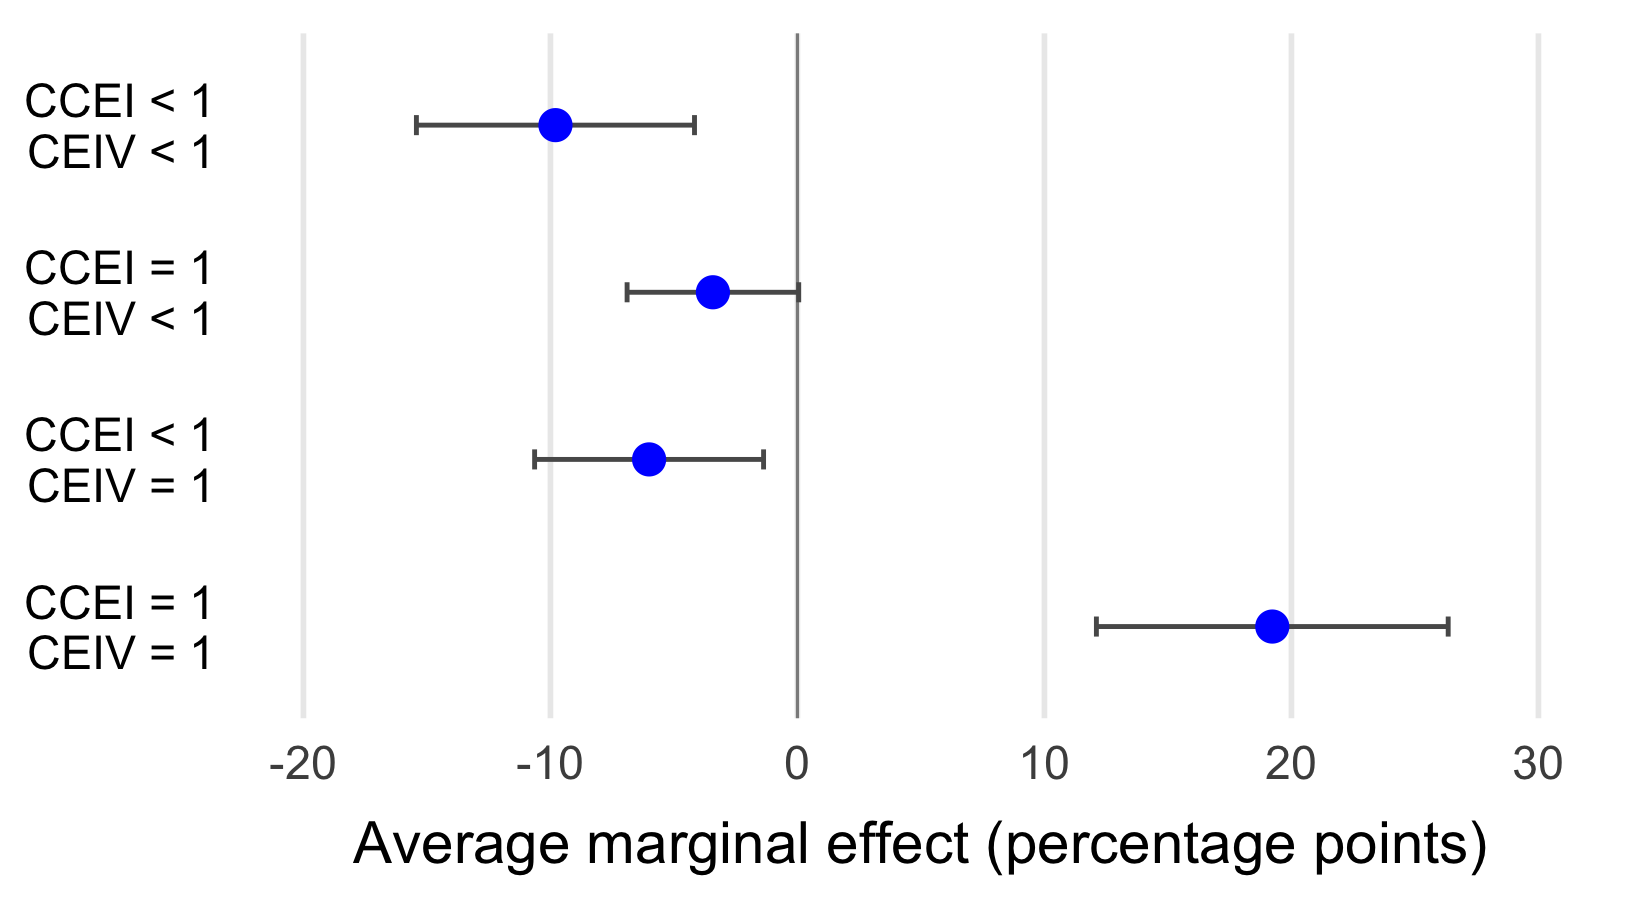
\includegraphics[width=\linewidth]{figure6_a_ame_maximum.png}\\
(a) $\mathrm{CCEI}_{\max,gt}$
\end{minipage}

\vspace{4pt}
\begin{minipage}{0.82\textwidth}\centering
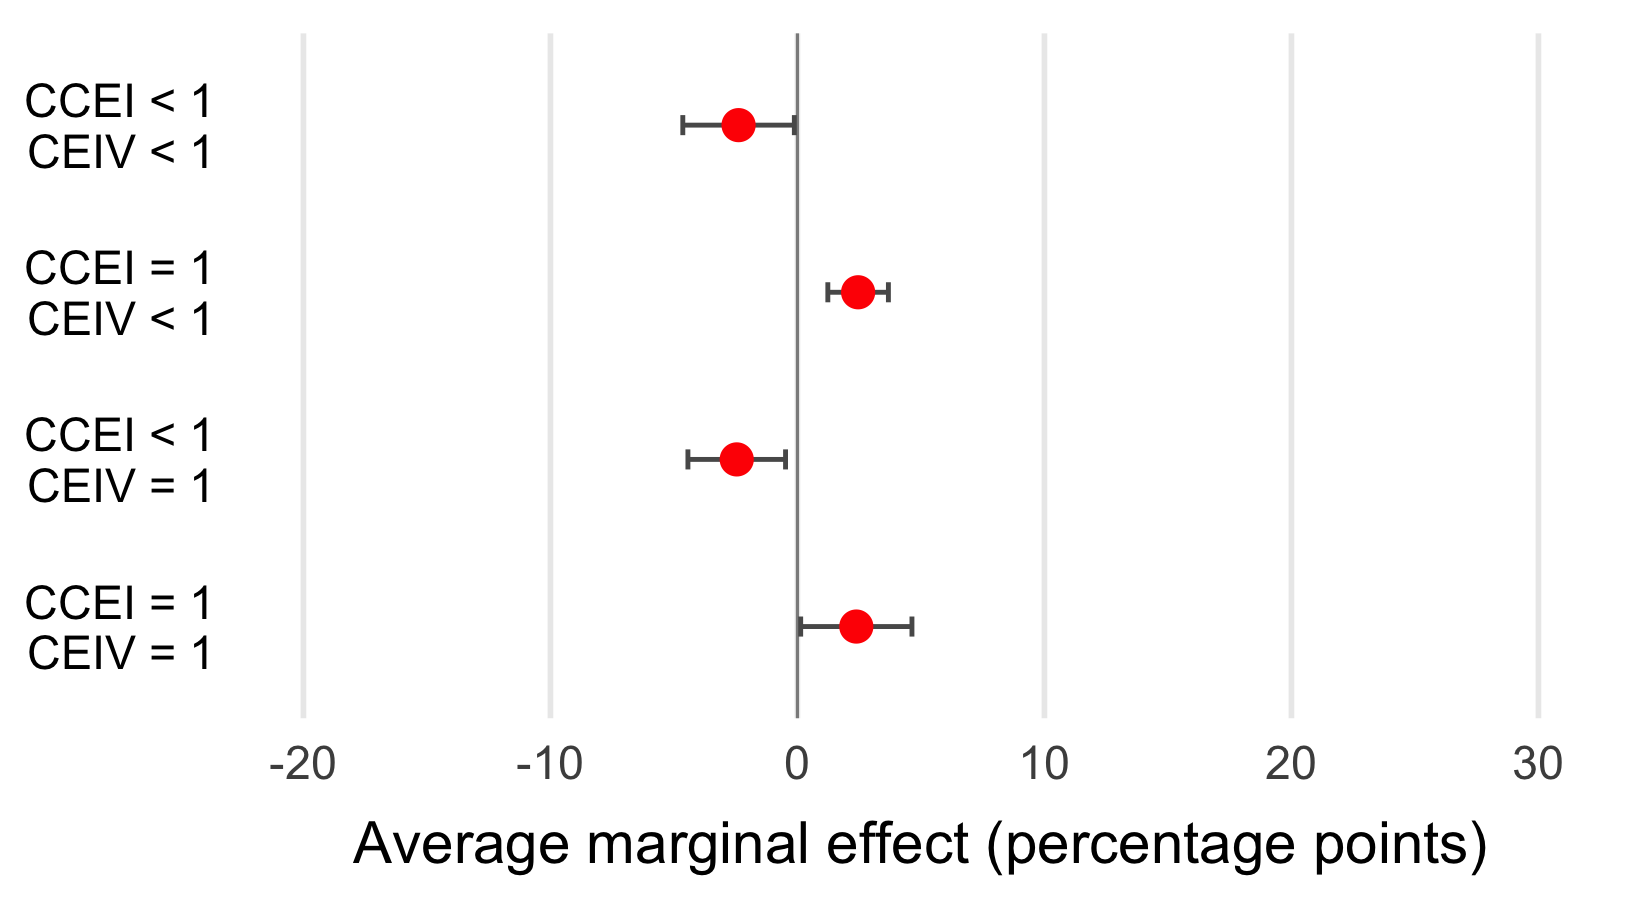
\includegraphics[width=\linewidth]{figure6_a_ame_minimum.png}\\
(b) $\mathrm{CCEI}_{\min,gt}$
\end{minipage}
\end{center}
\small
The four outcomes contain 415 pair-waves with both indices below one, 117 with only CCEI equal to one,
300 with only CEIV equal to one, and 472 with both equal to one.

\footnotesize
\textit{Notes:} This extension replaces CEI with CEIV in the four-outcome multinomial logit, matching the attached
Figure 6 variant. Both members' continuous CCEIs enter jointly, with all student, friendship, and corner/midpoint
share controls and class fixed effects, matching Column (5) of the expanded table. Risk-aversion controls and wave
fixed effects are excluded. The sample contains 1,304 pair-waves from 652 pairs, with 64 class clusters.
Dots report average marginal effects in percentage points, scaled to a 0.1 increase in the indicated member's CCEI;
these are scaled average derivatives, rather than exact finite changes in predicted probabilities.
Horizontal bars are 95\% normal intervals based on class-clustered standard errors. Effects sum to zero across
the four outcomes for each member. An index counts as one at values at least $1-10^{-9}$, and CEIV endpoint
classifications agree with both supplied numerical bounds. CEIV$=1$ indicates rationalizability under the specified
individual calibrations and varying weights; it does not identify actual aggregation weights or a communication
process. The effects are descriptive conditional associations.
\end{document}
